\chapter[Measurements]{Measurements}


The measurements can, to a certain extent, be broken into three main components: those pertaining to the solar wind, those from the magnetosphere in general, and those specific to the plasmasphere. An example of all the combined data sources is shown in Figure \ref{fig:alldata-GOES6-1983-1991}, providing solar wind variables $B_z$, $V_{SW}$; solar variable $F_{10.7}$, plasmatrough variable \req, and magnetosphere/plasmasphere variable \dst.

Similarly, Figure \ref{fig:alldata-GOES6-1989-1989} shows the same variables before, during, and after the March 1989 geomagnetic storm as seen by GOES 6. This makes it clearer how the variables are interrelated, notably how short-timescale effects such as drops in $B_z$ and \dst\ are connected, or longer time scale changes on $F_{10.7}$ and $V_{SW}$ are related. This figure also shows how the sparse availability of \req\ created challenges for this study, as discussed later.

\begin{figure}[htp!]
	\centering
	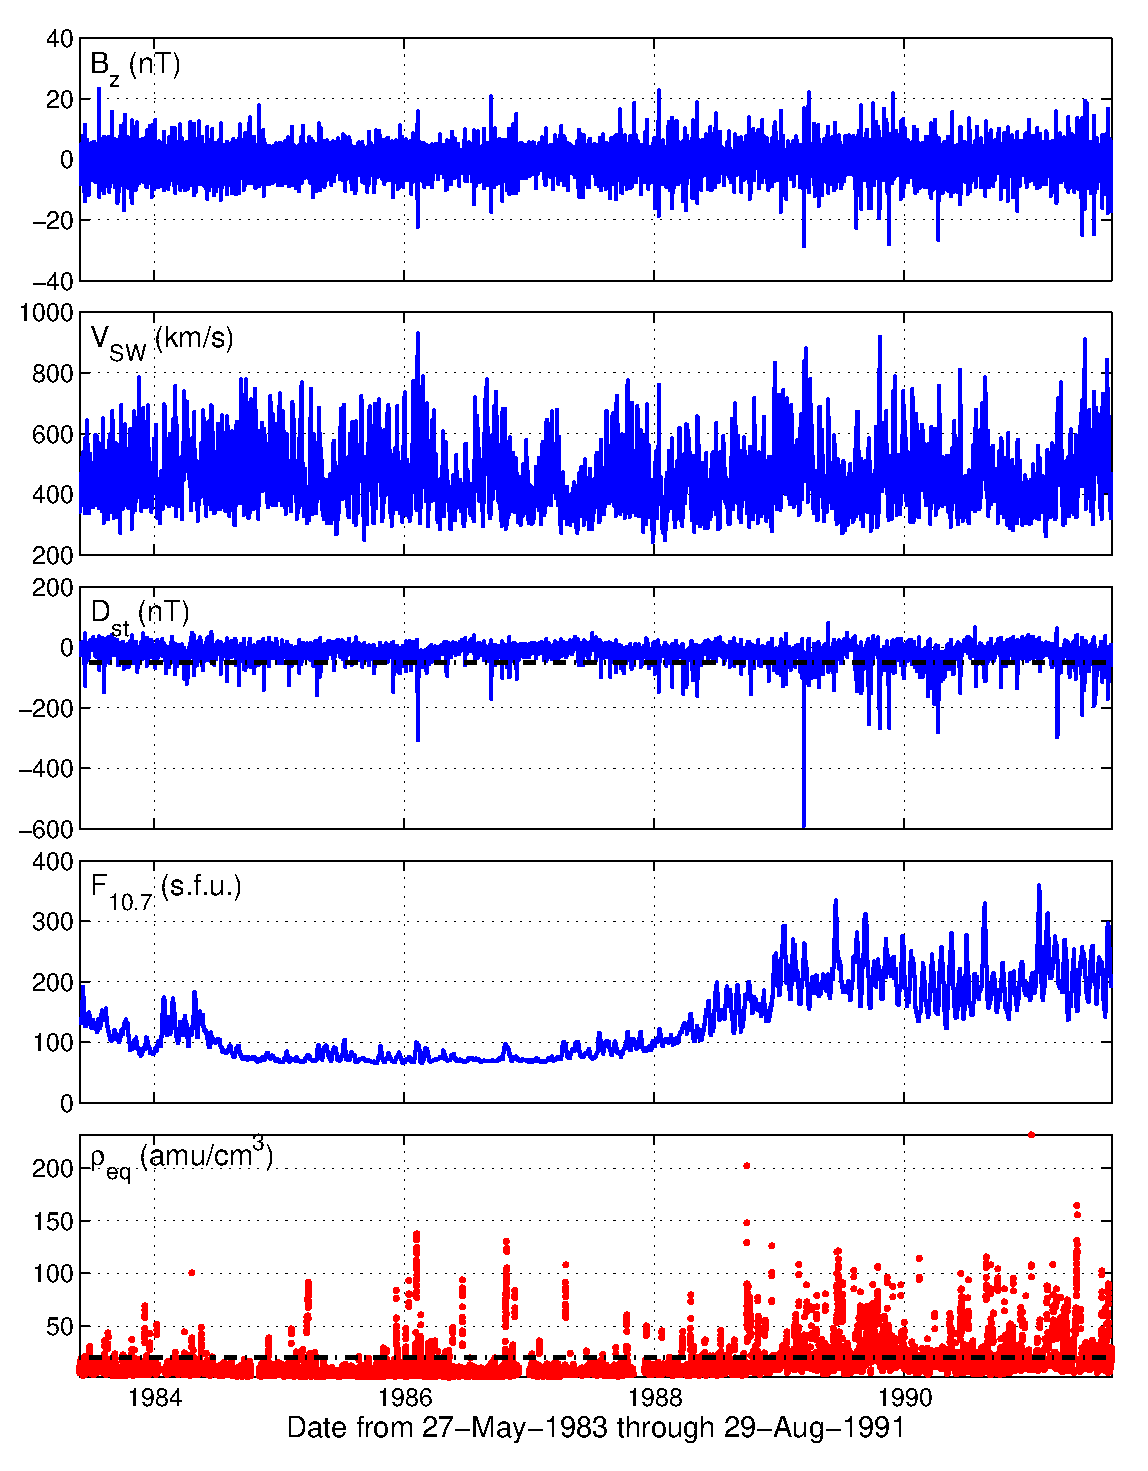
\includegraphics[width=0.7\linewidth]{Figures/alldata-GOES6-1983-1991}
	\caption{Data from GOES 6 with dashed lines indicating default storm thresholds}
	\label{fig:alldata-GOES6-1983-1991}
\end{figure}
\begin{figure}[htp!]
	\centering
	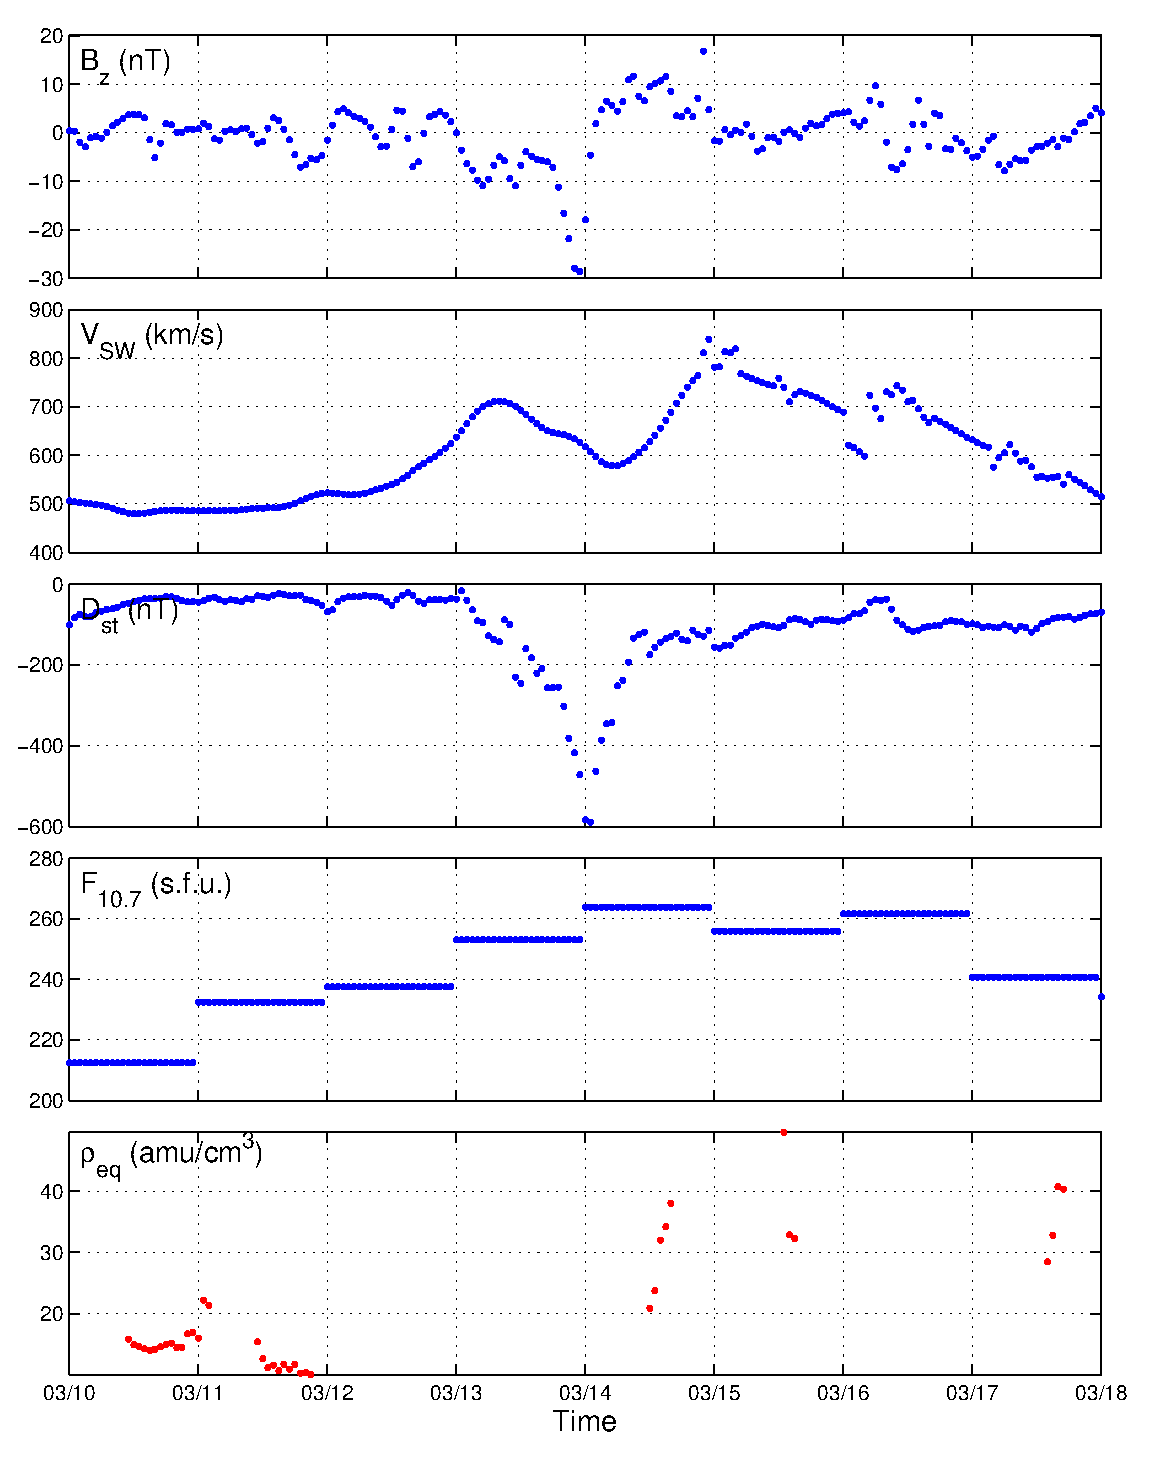
\includegraphics[width=0.7\linewidth]{Figures/alldata-GOES6-1989-1989}
	\caption{Data from GOES 6 around March 1989 geomagnetic storm}
	\label{fig:alldata-GOES6-1989-1989}
\end{figure}



\section{Solar Wind}
Solar wind is the largest driver of particle density in the magnetosphere \vinote{cite}, and as such is an important input for a plasmatrough model. Conditions such as magnetic field orientation and particle velocity are important considerations for whether the plasmasphere is expected to be compressed, saturated, or experiencing high variability. By adding these to a model that account for time delayed inputs, their effects can be accounted for and aid in categorizing the state of the plasmatrough.

\subsection{Source}
Solar wind data for this dissertation is provided by the OMNIWeb service \vinote{cite}, a combination of many satellites' data to create a uniform, high resolution, near-Earth set of solar wind measurements. The one-hour resolution dataset was used since the study is concerned with effects on timescales of longer than an hour, and to more easily compare to the other data sources used. 

However, since the OMNIWeb data has gaps for some of the variables, \cite{Kondrashov2014ReconstructionOfGaps} was used as they reliably reconstruct gaps to make a continuous, uniform data set. They used Singular Spectrum Analysis with synthetic gaps created by shifting real gaps from 1984-1995 data onto 1996-2007 data so that verification data would exist to test the effectiveness of their model. 

\subsection{Coverage}
Low resolution OMNI data is available from 1963 to present, but only the years of 1983-1992 were considered as they overlapped with the other data sets of interest. The data covers, but is not limited to: magnetic field strength in all three dimensions; solar wind proton density and temperature; the $K_p$, $AE$, $F_{10.7}$, and $D_{st}$ indices; and varying levels of proton flux.

\subsection{Data preparation}
The only data cleaning required on the OMNI dataset was to convert fill values of 999.9 and 9999 to NaN, to be appropriate for use in data analysis. Of the variables included (see Coverage), $B$, $B_z$ (GSE and GSM), and Solar wind proton density and plasma speed all were missing about 35\% of their data. The $AE$ index was missing about 7\% of its data, and all other variables were provided complete.

\section{Geomagnetic}
Geomagnetic data cover everything inside the magnetopause, but in this study will tend to refer specifically to information in the magnetosphere but not in the plasmasphere or ionosphere.

\subsection{Source}
The data come from \cite{Takahashi2010SolarCycleVariation}, which takes data from the Geostationary Operational Environmental Satellites (GOES) and uses a set of magnetic field models to relate Alfvén waves to equatorial mass density (\req). By taking magnetic field vectors and applying spectral analysis, they find a set of fundamental harmonic frequencies of toroidal waves. Through testing, they find a strong linear dependence of the 27-day average third toroidal frequency ($f_{T3\_27d}$) on the similarly averaged $F_{10.7}$ index, of the form: $f_{T3\_27d}(mHz)=37.5-0.0972 F_{10.7\_27d}(sfu)$. From there, they also find a linear relationship to the averaged \req\ in the form $log(\rho_{eq\_27d})=0.421+0.00390 F_{10.7\_27d}$, effectively linking the derived toroidal frequency to \req.

\subsection{Coverage}
The GOES satellites used in this study cover the years from 1980 to the end of 1991, often with overlapping years between satellites. The satellites themselves held a geostationary orbit at around 6.62 $R_E$ and collected data on a roughly 3-second cadence \citep{GOESDataSource}, which was then transformed onto a 10-minute cadence. Their position means they're almost always measuring properties of the plasmatrough, the region devoid of dense plasma just outside the plasmasphere.

\subsection{Data preparation}
The data were prepared by replacing fill values of 9999 with NaN and then narrowing results to only one satellite at a time to ideally remove any effects of satellite position or calibration from the results. These data still had many temporal gaps, so they were scaled onto a uniform 10-minute grid leaving missing points as NaN, but allowing for easier data analysis and comparison to other data sets.

In order to align the GOES data with the OMNI 1-hour cadence, the median of all existing values within 30 minutes on either side of each hour was taken. For hours with no existing values, a NaN was inserted to keep the cadence uniform. Two other methods were attempted: using the mean of each hour, centered on the hour, and using the median of the data on or within an hour after each time point (e.g. 7:00-7:59 would be combined into the 7:00 point). Both were found to have minimal effect on results.

\section{Plasmasphere}
Plasmasphere data covers the inner regions of the magnetosphere, bounded by the plasmapause on the outer edge and the ionosphere on the inner edge. This puts it at a typical distance of $L=3-5R_E$. 

\subsection{Source}
Data for the plasmasphere also comes from the GOES and OMNI datasets previously discussed, but are often calculated as extensions of directly measured data either onboard the satellites or from ground stations, depending on the current extent of the plasmasphere and location of the satellite.

\subsection{Coverage}
Since the data come from the same sources as that of the magnetosphere, the coverage is largely the same with specifics covered in \cite{Takahashi2010SolarCycleVariation}, where any error associated with temporary conditions is overshadowed by the variance in effectiveness of the model itself. 

\subsection{Data preparation}
The same preparation done for the magnetosphere applied to the plasmasphere data.  Some specific analysis done in \cite{Takahashi2010SolarCycleVariation} discusses how the spacecraft's geomagnetic location affected their ability to detect the necessary toroidal frequency, and thus estimate \req, so for some of the long-timescale averages, only certain MLTs were included. They also show that \req\ inversely correlates with geomagnetic activity (and, by extension, plasmapause location), so during long periods of no activity the plasmasphere extends beyond geosynchronous orbit, leading to measurements of \req\ reflecting density in the plasmasphere and not the plasmatrough. 
